\documentclass[a4paper]{article}

%--------------------------------------------------------------------------
\usepackage[a4paper, total={6in, 9in}]{geometry}
\usepackage{amsmath}
\usepackage{booktabs}
\usepackage{caption}
\usepackage{enumitem}
\usepackage{graphicx}
\usepackage{float}
\usepackage{inconsolata}
\usepackage{listings}
\usepackage{siunitx}
\usepackage[most]{tcolorbox}

%--------------------------------------------------------------------------
\graphicspath{{./fig/}}

%--------------------------------------------------------------------------
\begin{document}
\title{Udacity: Robotic Arm Pick \& Place Report}
\author{Shane Reynolds}
\maketitle

%--------------------------------------------------------------------------
\section{Introduction \& Background}
The Amazon Pick and Place Robotics Challenge is a competition designed to help increase collaboration between the industrial and robotics research communities. Amazon has successfully implemented a number of robotic systems which largely eliminate the need for activities like searching and walking in their fulfilment centres, however, one of the main challenges that Amazon is yet to solve is picking and stowing objects reliably in an unstructured environment. To successfully achieve this objective, there are a number of tasks that need to be successfully completed. These include:
\begin{enumerate}
\item Identification of the target object in the unstructured environment;
\item Manipulator path planning to the object;
\item Successful execution of a reach and grasp manoeuvre; and
\item Physical relocation of the grasped object to the desired location.
\end{enumerate}

\begin{figure}[h]
\centering
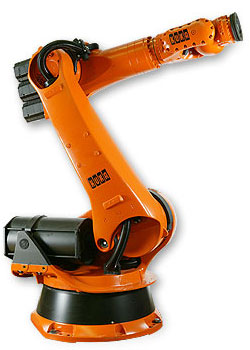
\includegraphics[scale=0.5]{image1}
\caption{Kuka KR210 anthropomorphic industrial robot with 6 degrees of freedom}
\end{figure}

Path planning and execution of the desired manoeuvre is largely a solved problem. The move execution is dependent on a field of robotics called inverse kinematics. The inverse kinematics (IK) of a robot is the mathematical conversion of position in Cartesian space to the joint angles which allows the robot end effector to reach the desired position. Briefly, the end effector position in space can be thought of in 2 separate domains: Cartesian world coordinates, or Joint Angle space. Typically, analytical work is done in Cartesian space - three dimensional space is the native environment that humans live in and is easier to conceptualise. Robots, however, position themselves by making adjustments to electrical or hydraulic actuators - these actuators receive instructions based on Joint Angle. This project explores the IK derivation, and implementation, for the Kuka KR210. The KR210 is a 6 degree of freedom (dof) anthropomorphic robotic arm shown in Figure 1. The project culminates with the implementation of an IK server, which is a ROS service receiving a series of points in Cartesian space (world coordinate frame), and returning a vector of Joint Angles after applying the IK transform. The implementation will be undertaken in ROS, which utilises simulation engines Rviz and Gazebo. Figures 2 and 3 show the Kuka KR210 in simulation.

\begin{figure}[h]
\centering
\begin{minipage}{0.45\linewidth}
\centering

\includegraphics[scale=0.5]{placeholder}
\caption{Include a picture of the KR210 in Gazebo}
\end{minipage}
\hspace{0.5cm}
\begin{minipage}{0.45\linewidth}
\centering

\includegraphics[scale=0.5]{placeholder}
\caption{Include a picture of the KR210 in Rviz}
\end{minipage}
\end{figure}

%--------------------------------------------------------------------------
\section{Methods \& Implementation}

\subsection{Determining the Denavit-Hartenburg Parameters}
Forward and Inverse kinematic analysis relies heavily on successful specification of transformation matrices between the physical elements of the robot, which we call links. In order to determine these transformation matrices, we need to assign coordinate frames to the robot links. Doing this in an arbitrary fashion will often result in the determination of 6 parameters for each transformation matrix, which makes this process undesirably complex. Denavit and Hartenburg (1955) determined an algorithmic approach to the assignment of coordinate frames to the robot's links which reduces the number of parameters needed to describe each transformation matrix to 4. Assuming that $\hat{x}_i$, $\hat{y}_i$, and $\hat{z}_i$ are the $x$, $y$, and $z$ axes respectively for coordinate frame $i$, then these parameters are defined in Table 1.

\begin{table}[h]
\centering
\caption{text}
\begin{tabular}{cp{8cm}}
\toprule
\textbf{Parameter} & \textbf{Description}\\
\midrule
$\alpha_{i-1}$ & Twist angle, and is determined by the angle between the $\hat{z}_{i-1}$ and $\hat{z}_i$, measured about the $\hat{x}_{i-1}$ axis\\
 & \\
$a_{i-1}$ & Distance from $\hat{z}_{i-1}$ to $\hat{z}_i$ measured along $\hat{x}_{i-1}$, where $\hat{x}_{i-1}$ is orthogonal to $\hat{z}_{i-1}$, and $\hat{x}_{i-1}$ is orthogonal to $\hat{z}_i$\\
 & \\
$d_i$ & Signed distance between $\hat{x}_i$ and $\hat{x}_{i-1}$, measured along $\hat{z}_i$\\
 & \\
$\theta_i$ & \\
\bottomrule
\end{tabular}
\end{table}
  
\subsection{Forward Kinematics}
Forward kinematics is the transformation of joint angles to an end effector point in space. Provide an in depth description of how each of the transformations and how they were arrived at. Recall this is a simple implementation of the DH parameter matrices and then a simple multiplication (which can be done using sympy)

The individual transformation matrices are shown below:
\begin{align*}
	^\texttt{base\_link} T_1 &= MATRIX ARRAY\\
	^1 T_2 &= MATRIX ARRAY\\
	^2 T_3 &= MATRIX ARRAY\\
	^3 T_4 &= MATRIX ARRAY\\
	^4 T_5 &= MATRIX ARRAY\\
	^5 T_6 &= MATRIX ARRAY\\
	^5 T_\texttt{end\_effector} &= MATRIX ARRAY
\end{align*}

The full transformation from the \verb|base_link| to the \verb|end_effector| is given by simple matrix multiplication as follows:
\begin{align*}
	^{\texttt{base\_link}} T_{\texttt{end\_effector}} &= ^{\texttt{base\_link}} T_{1} \cdot ^{1} T_{2} \cdot ^{2} T_{3} \cdot ^{3} T_{4} \cdot ^{4} T_{5} \cdot ^{5} T_{6} \cdot ^{6} T_{\texttt{end\_effector}}
\end{align*}

\subsection{Inverse Kinematics}
Inverse kinematics is the process of determining the joint angles for each of the degrees of freedom. In the case of the Kuka XXXX there are 6 degrees of freedom, and hence, there are 6 joint angles which need to be determined. The anthropomorphic arm design allows us to exploit the fact that the last 3 joints are a spherical wrist (their axes of rotation intersect?), which means that these joints do not have an influence on the position of the wrist centre. This allow us to kinematically decouple the the first three joints and the last three joints, providing the ability to find a closed form solution to the problem. The closed form solution is presented below, in two parts: first three joint angles, and final three joint angles

\subsubsection{First Three Joint Angles ($\theta_1$, $\theta_2$, and $\theta_3$)}
Mathematics to show the derivation of the first three angles

\subsubsection{Final Three Joint Angles ($\theta_4$, $\theta_5$, and $\theta_6$)}
Mathematics to show the derivation of the final three angles

%--------------------------------------------------------------------------
\section{Results \& Conclusion}
Discussion of the results of the robot kinematics.

%--------------------------------------------------------------------------
\section{Further Enhancements}
The wrist turns around a bit - need to make sure that this doesn't happen and why this is happening. It happens because the wrist has more that 360 twist capability, however, the way it is set up does not allow for this (it has hard clamps at $-\pi$ and $\pi$). Also an error tracking capability would be nice on the project also.

\end{document}